%==============================================================================
% Sjabloon poster bachproef
%==============================================================================
% Gebaseerd op document class `a0poster' door Gerlinde Kettl en Matthias Weiser
% Aangepast voor gebruik aan HOGENT door Jens Buysse en Bert Van Vreckem

\documentclass[a0,portrait]{hogent-poster}

% Info over de opleiding
\course{Graduaatsproef}
\studyprogramme{Graduaat in het Programmeren}
\academicyear{2024-2025}
\institution{Hogeschool Gent, Valentin Vaerwyckweg 1, 9000 Gent}

% Info over de bachelorproef
\title{C++ en Unreal Engine}
\subtitle{C++ verkennen met gamedev}
\author{Sheylene Bos}
\email{sheylene.bos@student.hogent.be}
\supervisor{Luc Vervoort}
\cosupervisor{}

% Indien ingevuld, wordt deze informatie toegevoegd aan het einde van de
% abstract. Zet in commentaar als je dit niet wilt.
\specialisation{Programmeren}
\keywords{C++, Unreal Engine, gamedev}
% Uncomment the next line only if \projectrepo is defined in your document class or preamble
% \projectrepo{https://dev.azure.com/GraduaatsProefSheylene/_git/theystillremain}
% ```

\begin{document}

\maketitle

\begin{abstract}
C++ is een intressante taal die meer dan 40 jaar bestaat, daarom heb ik ervoor gekozen.
Tijdens de ontwikkeling waren er een paar uitdagingen, zoals het leren van de taal en het werken met Unreal Engine 5.
Het project is meer een demo dan een volledig spel, maar het heeft me geholpen om de taal en de engine beter te begrijpen.
Het doel van deze graduaatsproef is om C++ te leren kennen en de verschillen met C\#, een taal die we tijdens de opleiding hebben geleerd, te ontdekken.

\end{abstract}

\begin{multicols}{2} % This is how many columns your poster will be broken into, a portrait poster is generally split into 2 columns

\section{Introductie}

C++ is een invloedrijke programmeertaal die al meer dan 40 jaar bestaat en nog steeds populair is voor systeemsoftware en game-ontwikkeling. Deze graduaatsproef verkent C++ binnen de context van Unreal Engine 5, een moderne game-engine van Epic Games bekend om zijn geavanceerde grafische technologieën zoals Nanite en Lumen.

De keuze voor C++ en Unreal Engine 5 is gedreven door de wens om de kracht en complexiteit van C++ te ervaren in een creatieve omgeving. Het hoofddoel is om C++ te leren kennen en de verschillen met C\#, een taal uit de opleiding, te ontdekken.

\section{Ontwikkeling}

De ontwikkeling in C++ en Unreal Engine 5 bracht diverse uitdagingen met zich mee. Het correct opzetten van het project, inclusief header (.h) en source files (.cpp), en het begrijpen van het compilatieproces naar object files (.o, .obj) was een eerste stap. Anders dan C\# met zijn \texttt{using}-directive, vereist C++ het gebruik van \texttt{\#include} voor header files, waarbij een onderscheid gemaakt wordt tussen eigen headers (" ") en standaardbibliotheken (<>).

Specifieke Unreal Engine-mechanismen, zoals de \texttt{UCLASS}-macro voor klassedefinities, vroegen gewenning. Problemen zoals het niet herkennen van klassen, wat soms een volledige herbouw van het project noodzakelijk maakte, en het correct toevoegen van klassen via de Unreal Engine Editor waren onderdeel van het leerproces. Ook het omgaan met de stabiliteit en laadtijden van de ontwikkeltools (Unreal Engine en Visual Studio) was een factor.

Er werd bewust gekozen om voornamelijk in C++ te programmeren om de taal diepgaand te leren, en Blueprints voornamelijk voor visuele representatie te gebruiken. Dit betekende het zelf schrijven en doorgronden van code in plaats van het blindelings volgen van tutorials.

Om de code gestructureerd en onderhoudbaar te houden, zijn design patterns toegepast. De Simple Factory Pattern werd gebruikt voor het creëren van items zoals wapens en voedsel. De Observer Pattern zorgt ervoor dat de gebruikersinterface (UI) up-to-date blijft met spelerinformatie, en de Factory Method Pattern is ingezet voor het genereren van verschillende types vijanden. Daarnaast is er een inventory systeem geïmplementeerd.

\section{Sectie met figuur}

De {\LaTeX} figure-omgeving bepaalt zelf waar een afbeelding komt en dat is meestal niet op de plek in de tekst waar de figure-omgeving gedefinieerd wordt. Als je wilt forceren dat afbeeldingen toch in de flow van de tekst blijven, dan kan je dat zoals hieronder:

\begin{center}
  \captionsetup{type=figure}
  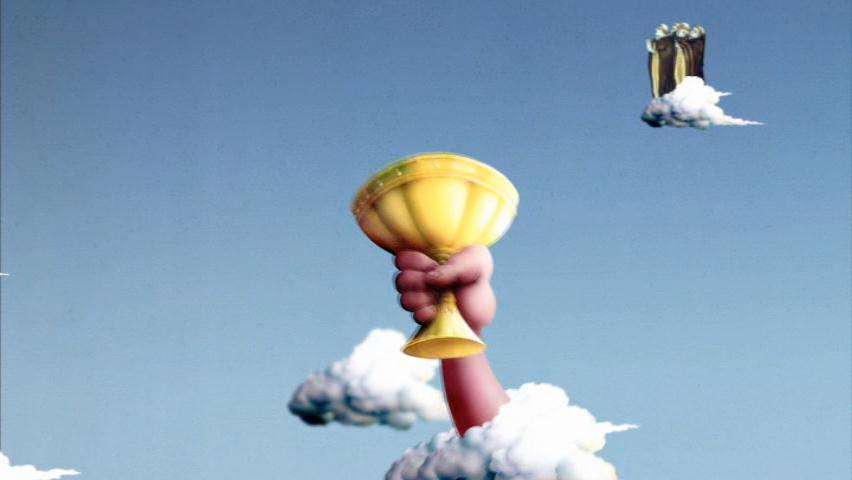
\includegraphics[width=1.0\linewidth]{grail}
  \captionof{figure}{He hasn't got shit all over him. The nose? Where'd you get the coconuts? What do you mean? We shall say `Ni' again to you, if you do not appease us}
\end{center}

Let er wel op dat dit tot problemen met bladschikking kan leiden.

\section{Conclusies}

Het starten van dit project was een uitdaging, mede door een gebrek aan voorkennis van C++ en Unreal Engine. Desondanks was het een leerzaam proces, waarbij vooral het onderzoek naar de achtergrond en evolutie van C++ als boeiend werd ervaren. Het project heeft doorzettingsvermogen en probleemoplossend vermogen vereist.

Hoewel de combinatie met Unreal Engine soms voor frustratie zorgde, met name door tijdsdruk en de visuele aspecten, was het leren van C++ zelf een positieve ervaring. De intentie is om in de toekomst verder te gaan met C++.

\section{Toekomstig onderzoek}

Verder onderzoek zou kunnen focussen op het dieper uitwerken van de game-mechanics in C++, het optimaliseren van de code voor betere prestaties, of het verkennen van meer geavanceerde Unreal Engine features. Verder kan het intressant zijn om vijanden AI te implementeren die gebruik maken van de eerder genoemde design patterns, zoals de Strategy Pattern voor verschillende bewegingspatronen. Ook kan er gekeken worden naar het uitbreiden van de game met meer complexe interacties en gameplay-elementen.
 

\end{multicols}
\end{document}